\section{Background} \label{sec:background}

% TBD.

\subsection{\paxos}\label{sec:paxos}
% \paxos background. Keys:
% Leader, backup.
% Persistent storage. 
% Network round trips in normal case. Latency.
An SMR system runs the same program and its data on a set of machines 
(replicas), and it uses a distributed consensus protocol (typically, 
\paxos~\cite{paxos:complex,paxos,paxos:simple,paxos:live,paxos:fast,
paxos:practical}) to coordinates inputs across replicas. For efficiency, in 
normal case, \paxos often lets one replica work as the leader which invokes 
consensus requests, and the other replicas work as backups to agree on or 
reject 
these requests. If the leader fails, \paxos elects a new leader from the 
backups.

% Two reliability features must be enforced in a standard \paxos protocol. The 
% first one is durability. When a new input comes, the \paxos leader writes this 
% input in local stable storage. The leader then starts a new consensus round, 
% which invokes a consensus request on ``processing this input" to the other 
% backups. A backup also writes the received consensus request in local storage 
% if it agrees on this request. Durability ensures that even if the leader or 
% backups fail and restart, they can still retrieve the requests from local 
% stable 
% storage and re-execute them.
% 
% The second feature is safety. As long as a quorum (typically, majority) of 
% replicas agree on this input (\ie, this input is \emph{committed}), \paxos 
% guarantees that all replicas consistently agree to process this input. If a 
% replica sees that an input consensus has been reached, this consensus must have 
% really been reached by at least a majority of replicas. Safety ensures that if 
% a consensus has not really been reached, no replica will ``think" that this 
% consensus has been reached.

% Durability and safety make replicas consistently agree on each input and 
% tolerate various faults, including machine failures and network errors. 

% As consensus rounds move on, \paxos consistently enforces the same sequence of 
% inputs across replicas. It also enforces same execution states across replicas 
% without divergence if a program behaves as a deterministic state machine (\ie, 
% always produces the same output on the same input).

% Normal case, round trip.
Network latency of consensus messages is one key problem to make general server 
programs adopt SMR. For instance, in an efficient, practical 
\paxos implementation~\cite{paxos:practical}, each input in normal case takes 
one consensus round-trip between every two replicas (one request from the 
leader and one reply from a backup).

\subsection{RDMA} \label{sec:rdma}

RDMA architecture such as Infiniband~\cite{infiniband} or RoCE~\cite{roce} 
recently becomes commonplace in datacenters due to its extreme low latency, 
high throughput, and its decreasing prices. 

RDMA provides three types of communication primitives, from slowest to 
fastest: IPoIB (IP over Infiniband), message verbs, and one-sided read/write 
operations. A one-sided RDMA read/write operation can directly write from one 
replica's memory to a remote replica's memory, completely bypassing OS kernel 
and CPU of the remote replica. For brevity, the rest of this paper denotes a 
one-sided RDMA write operation as a ``WRITE".


% \subsection{State Machine Replication (\smr)} \label{sec:smr}

% State machine replication (\smr) is a powerful fault-tolerance
% concept~\cite{paxos:practical}.  It models a program as a deterministic state 
% machine, where states are important program data and the transitions are 
% deterministic executions of program code under input requests.  \smr runs 
% replicas of this state machine on multiple nodes, tolerating many possible node 
% and network failures.  To keep the replicas consistent, it invokes a
% distributed consensus protocol (typically \paxos~\cite{paxos, paxos:simple, 
% paxos:practical}) to ensure that a quorum (typically majority) of the replicas 
% agree on the input request sequence; under the deterministic execution 
% assumption, this quorum of replicas must reach the same exact state.  \smr is 
% proven safe in theory, and provides high availability in practice.
% 
% To support general server programs transparently, \repbox leverages \repbox's 
% \paxos consensus protocol, which takes the POSIX socket API as
% consensus interface. This \paxos protocol enforces two kinds of 
% orders for socket operations. First, for requests coming from the clients, 
% such as \connect and \send requests, this protocol enforces that all nodes see 
% the same totally ordered sequence of these requests using the \paxos and socket 
% API interposition components.  (this protocol does not need to order the 
% blocking socket operations in the clients because we mainly focus on analyses 
% for server applications.) Second, for server applications' blocking operations, 
% this \paxos protocol schedules them according to the matching operations from 
% the clients (\eg, a \send from a client matches a \recv from the server within 
% the same socket connection). This protocol does not schedule non-blocking 
% operations in servers (\eg, \send to clients) because it focuses on replicating 
% the server's execution states.
% 
% % For practicality, \repbox's \paxos implementation takes a well-known 
% % engineering approach~\cite{paxos:practical}: only the primary invokes consensus 
% % request during normal operations, and an leader election is invoked when 
% % exceptions such as network partitions occur.
% 
% 
% Figure~\ref{fig:repbox} shows an instance of \repbox running on 
% each node, and the \paxos consensus component is the gateway of this instance.  This 
% component accepts socket requests from the clients and invoke a \paxos 
% consensus instance with the other replicas on this operation. Once a consensus 
% is reached, this component forwards the operation to the \dmt component. This 
% component is also the only \repbox component that communicates among different 
% \repbox instances. 
% 
% In this paper, \xxx skips the fault-tolerance nature of \repbox, but leverages it 
% to construct multiple equivalent executions for analysis tools.
% 
% \subsection{Deterministic Multithreading (\dmt)} \label{sec:dmt}
% 
% \dmt~\cite{dpj:oopsla09, 
% dmp:asplos09, kendo:asplos09, coredet:asplos10, dos:osdi10, ddos:asplos13, 
% ics:oopsla13} is an advanced threading technique that enforces the same 
% schedule 
% on the same inputs.  This technique typically maintains a \emph{logical
%   time}\footnote{Though related, the logical time in \dmt is not to be
%   confused with the logical time in distributed
%   systems~\cite{lamportclock}.} that advances deterministically based on
% the code run.  It allows a thread to synchronize only at deterministic
% logical times.  By induction, it makes an entire multithreaded execution
% deterministic.  The overhead of \dmt is typically moderate: one recent
% \dmt system, \parrot~\cite{parrot:sosp13}, incurs an average of 12.7\%
% overhead on a wide range of 108 popular multithreaded programs on 24-core
% machines.
% 
% The \dmt component in Figure~\ref{fig:repbox} runs within the same process as a server replica, and
% enforces the same logical clocks for inter-thread communication
% operations. \repbox leverages the \parrot~\cite{parrot:sosp13} \dmt runtime
% system because it is fast (\ie, 12.7\% overhead for a wide range of 108 popular 
% multithreaded programs) and transparent to the application.
% 
% 
% Specifically, \parrot uses a runtime technique called \ldpreload to dynamically 
% intercept \pthread synchronizations (\eg, \mutexlock) issued by an executable 
% and enforces a well-define, round-robin schedule on these synchronization 
% operations for all threads, practically eliminating nondeterminism in thread
% synchronizations. Although \parrot is not designed to resolve data races
% deterministically, deploying a race detector in one replica can overcome this 
% limitation (\S\ref{sec:discuss}).  \repbox augments the \dmt component to schedule 
% the return points of blocking socket operations in server replicas, too, to 
% ensure that requests are admitted exactly at the same logical time across 
% replicas.



% Our model. Multiple writer multiple reader.
\section{\xxx Overview} \label{sec:overview}

\begin{figure}[t]
\vspace{.20in}
\centering
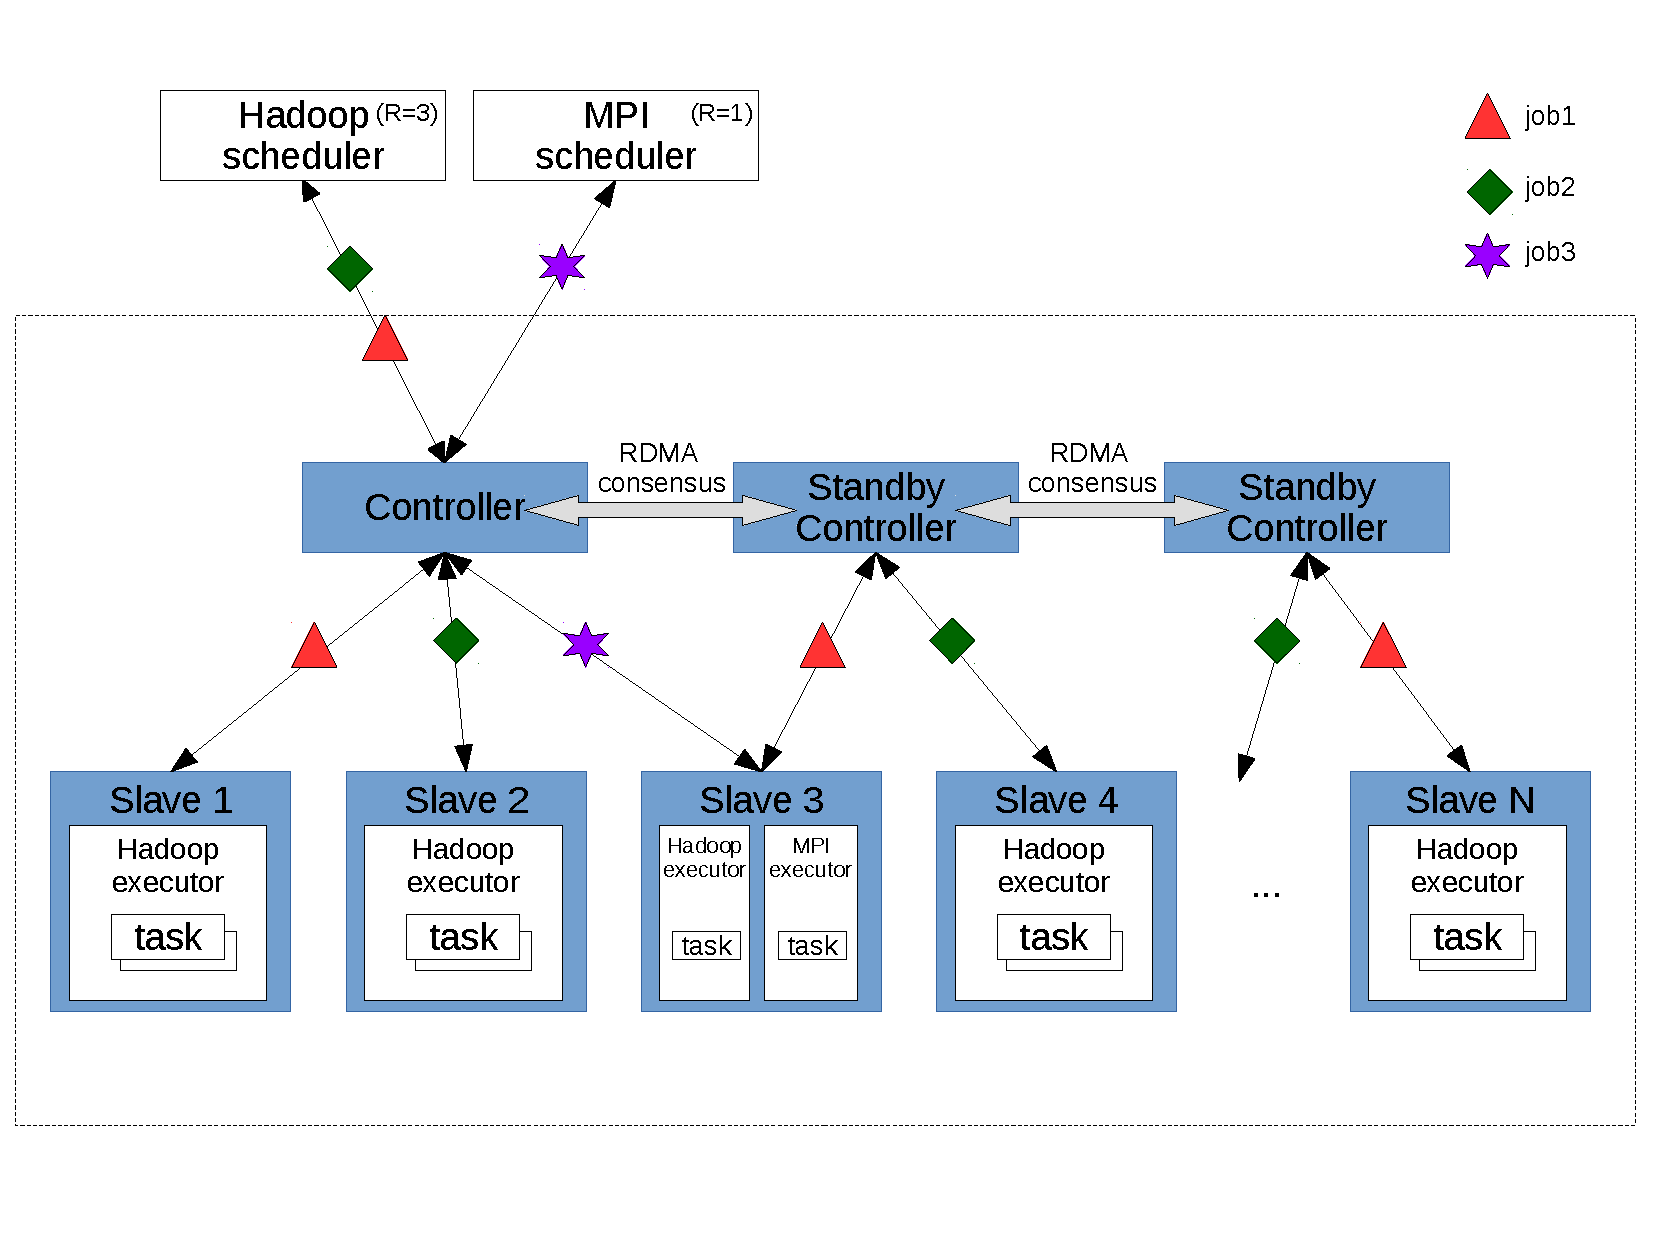
\includegraphics[width=.47\textwidth]{figures/arch}
\vspace{.06in}
\caption{{\em The \xxx Architecture.} Key components are shaded (and 
in green).} \label{fig:repbox}
\vspace{-.05in}
\end{figure}


TBD. 

\subsection{Architecture} \label{sec:arch}

TBD. 

\subsection{Workflow on Scheduling Tasks} \label{sec:workflow}

TBD. 

% \xxx's deployment model is similar to \repbox's except two things: (1) at least \v{f}+1 nodes 
% run an actual execution or a lightweight analysis tool on 
% each so that they can reach consensus on inputs and process requests fast, and 
% (2) at most \v{f} nodes run an heavyweight analysis tool on each. Empirically 
% (see \S\ref{sec:eval}), this paper considers an analysis tool with no more than 30\% overhead as 
% lightweight tools (\eg, DynamoRio's drcov tool~\cite{dynamorio}), while the other tools heavyweight 
% tools (\eg, the Helgrind race detector~\cite{valgrind:pldi}).
% 
% A \xxx instance running on each node is the same as the one in 
% Figure~\ref{fig:repbox} except that a server program runs transparently in a \xxx instance 
% with or without an analysis tool. Neither the server or the analysis is aware of \xxx's 
% components. The remaing of this section first presents \xxx's checkpoint and 
% rollback design for analysis tools (\S\ref{sec:checkpoint}), and discusses \xxx's potential 
% benefits (\S\ref{sec:discuss}).

% \subsection{Checkpoint and Rollback Mechanism} \label{sec:checkpoint}
% 
% To allow synchronous analysis tools (\eg, control flow integrity and buffer 
% overrun protection tools) to recover from malicious events, we have designed a 
% checkpoint mechanism for \xxx. Each checkpoint is associated with the index of the last 
% executed socket operation, so that \xxx can consistently match up with the execution 
% states of native executions and various analysis executions.
% 
% To perform checkpoints transparently without affecting application's executions and analyses, \xxx 
% leverages \criu~\cite{criu}, a popular, open source process checkpoint tool 
% that supports CPU registers, memory, etc. Each checkpoint operation is only performed on the 
% server program and the \dmt scheduler; the \paxos consensus component does not 
% require checkpoints because we explicitly design it to be stateless (all socket 
% operations have been persistently logged). 
% 
% \xxx provides two functions, one for checkpoint and the other for rollback.
% When an analysis tool calls the \v{checkpoint()} function, \xxx uses 
% its \paxos consensus component to invoke an operation: ``take a checkpoint 
% associated with the global index of the latest socket operation". Once a 
% consensus is reached, all replicas (including primary) do a checkpoint 
% operation as the next consensus operation.
% 
% 
% When the tool catches a malicious event and decides to roll back to a previous
% checkpoint associated with a socket operation index, the tool calls a 
% \v{rollback(int} \v{index=-1,} \v{bool discard=true)} function. Ignoring the 
% arguments in this function means rolling back to the last checkpoint within all 
% replicas and discard all inputs since this checkpoint. This API works as three 
% steps: (1) current replica uses the \paxos consensus component to request an 
% operation: ``rollback to a previous checkpoint according to \v{index}"; (2) 
% once consensus is reached, each replica invokes \criu to do the actual rollback 
% operation; (3) if \v{discard} is on, each replica discards all future inputs 
% since the checkpoint. Overall, this API makes all replicas rollback and discard 
% malicious inputs consistently.
% 
% 
% \xxx's checkpoint mechanism has a few limitations: (1) although this mechanism's 
% API is expressive, they moderately trade off transparency between an analysis 
% tool and \xxx's framework; (2) it may defer the processing of network requests; 
% and (3) it can not revoke information that have already leaked to clients. 
% However, considering the benefits (\S\ref{sec:strengthen-analysis}) that \xxx 
% may bring to tools, we argue that this checkpoint mechanism is still worthwhile.
% 
% 
% \subsection{Discussion} \label{sec:discuss}
% 
% \subsubsection{What Types of Analyses are Suitable to Run in \xxx?} 
% \label{sec:analysis-types}
% 
% We envision that an analysis can transparently run in \xxx if: (1) it can run 
% asynchronously with the actual execution, and (2) it does not schedule 
% conflicting order of \pthread synchronizations that \xxx's \dmt runtime 
% enforces. Many reliability analyses (\eg, data race detection), profiling, 
% and logging tools meet this requirement.
% 
% Some synchronous security analysis such as control 
% flow integrity can not transparently run in \xxx because it monitors the 
% execution 
% synchronously for each control flow transfer. In addition, some other security 
% analysis such as information leakage protection can not transparently run in 
% \xxx 
% because the actual execution may probably run faster than the 
% analysis and leak information to clients before the analysis detects the 
% leakage. Nevertheless, many security tools such as use-after-free 
% vulnerabilities can be transparently deployed in \xxx. If a synchronous 
% analysis 
% tool would like to run in \xxx, it should use \xxx's checkpoint 
% and rollback APIs (\S\ref{sec:checkpoint}).
% 
% 
% \subsubsection{Can \xxx Strengthen Existing Analyses?} 
% \label{sec:strengthen-analysis}
% 
% \xxx has the potential to strengthen existing analyses via its performance 
% benefit. Previously, to mitigate the huge performance slowdown, some analysis 
% tool developers sometimes have to weaken the guarantees of an analysis. For 
% instance, ThreadSanitizer\cite{tsan}, one of the most practical race detectors, 
% only logs the last four accesses for each memory byte instead of the complete 
% access history, because logging and analyzing the complete history is quite 
% heavyweight (\eg, 20X+ slowdown for some testing programs the authors 
% evaluated). However, an incomplete access history may miss data races at 
% runtime. With \xxx, developers can now strengthen the analysis by logging 
% complete memory access history.
% 
% \xxx also has the potential to speedup existing analysis tools themselves via 
% its replication architecture. For instance, the high logging overhead for 
% failure reproductions on multi-processors is an open research 
% problem~\cite{sherlog:asplos10}. Fortunately, with \xxx's architecture, these 
% logging tools now can separate different logging aspects such as functions, 
% libraries, and threads into different replicas (\eg, each replica logs for only 
% one thread), greatly reducing the logging overhead. Sampling-based race 
% detection tools (\eg,~\cite{datacollider:osdi10}) can also greatly reduce 
% sampling overhead by dividing sampling work into replicas, or can significantly 
% multiply sampling rates by running the same tool among replicas.
% 
% Moreover, \xxx provides an extra fault-tolerance benefit for analysis tools. 
% Existing reliability and security analyses tend to expose or detect harmful 
% defeats in an application, which may crash the application. In addition, the 
% actual executions across different nodes may fail as well due to hardware or OS 
% failures. With \xxx's \smr architecture, the sequence of inputs are 
% persistently and consistently enforced across replicas, and failing minor 
% nodes (either an analysis or an actual execution node) do not affect the other 
% nodes' executions and analyses.
% 
% % \subsection{Can \xxx Speedup Existing Analyses?} 
% % \label{sec:speedup-analysis}
% % 
% % TBD.
% 
% \subsubsection{Can Existing Analyses Benefit \xxx?} 
% \label{sec:strengthen-crane}
% 
% Interestingly, analyses running in \xxx can benefit \xxx's \dmt runtime and 
% improve \xxx's performance. Existing typical \dmt systems use two approaches to 
% enforce schedules. First, a \dmt approach enforcing a total order order for 
% shared memory accesses (for short, mem-schedules) is fully deterministic even 
% with data races, but this approach incurs prohibitive slowdown. For instance, 
% \dthreads~\cite{dthreads:sosp11} incurs several times slowdown for many 
% programs because typical applications have intensive amounts of shared memory 
% accesses.
% 
% The other \dmt approach is enforcing a total order for 
% synchronizations only (for short, sync-schedules). This approach can be 
% efficient because most code is not synchronization and can still run in 
% parallel. For instance, \kendo, \tern, and \peregrine~\cite{kendo:asplos09, 
% cui:tern:osdi10, parrot:sosp13} incurred less than 16\% overhead on most 
% programs they evaluated. However, this approach is only deterministic when 
% no races occur. Overall, despite much effort~\cite{dthreads:sosp11, 
% parrot:sosp13, peregrine:sosp11, determinator:osdi10}, an open problem still 
% exists: people lack a simple and deployable approach to enforce fully 
% deterministic and efficient \dmt schedules.
% 
% 
% Fortunately, \xxx's replication architecture can address this problem by simply
% running a race detector in one replica, then \xxx can choose the faster \dmt 
% approach that enforces sync-schedules. If the race detector reports a race, 
% application developers can easily diagnose and fix it because synchronization 
% schedules enforced by \dmt already make races easily 
% reproducible~\cite{pres:sosp09}. By enforcing the same synchronization 
% schedules across replicas, race detection results consistently hold for all 
% replicas. In sum, \xxx and race detection tools form a mutually beneficial 
% eco-system.

% \section{Replication-aware Scheduling} \label{sec:algo}
% \begin{algorithm}[t]

\DontPrintSemicolon

%\SetCommentSty{textrm}

\small

\SetCommentSty{textrm}

\SetKwInOut{Input}{Input}\SetKwInOut{Output}{Global}
\Input{program $prog$, initial state $s_0$, checker $checker$}
\Output{state queue $q$, branch tree $brtree$}

\SetKwBlock{Titlea}{RuleDirectedSE($prog$, $s_0$, $checker$)}{end}
\Titlea {
  $q$.add($\langle s_0, prog$.entry$\rangle$) \;
  \While {{\rm $q$ not empty {\bf and} time limit not reached}} {
    $\langle s, i \rangle$ $\leftarrow$ $q.$remove() \;
    \If {{\rm $i$ is not a symbolic branch statement} {\bf or}
        {\rm only one branch is feasible}} {
      $\langle s', i' \rangle$ $\leftarrow$ run($s$, $i$) \;
      HandleNewState($s$, $i$, $s'$, $i'$, $checker$) \;
    } \Else(\tcp*[h]{fork states and add constraints}) {
      $s_{true}$ $\leftarrow$ $s + \{$$i$.cond = true$\}$ \;
      $s_{false}$ $\leftarrow$ $s + \{$$i$.cond = false$\}$ \;
      \nlset{*} $brtree$.add($i$, $s_{true}$, $s_{false}$) \;
      HandleNewState($s$, $i$, $s_{true}$, $i$.true\_br, $checker$) \;
      HandleNewState($s$, $i$, $s_{false}$, $i$.false\_br, $checker$) \;
    }
  }
}

\SetKwBlock{Titlea}{HandleNewState($s$, $i$, $s'$, $i'$, $checker$) \tcp*[h]{Note: $s'$
    is updated}}{end}
\Titlea {
  \nlset{*} \If {{\rm {\bf not} $checker$.OnExecution($s$, $i$, $evmask$)}} {
    \nlset{*} \Return \tcp*[h]{error detected!} \;
  }
  \nlset{*} $s'$.path.push\_back($i$) \;
  \nlset{*} \If {$evmask$ $\neq$ 0} {
    \nlset{*} $s'$.events.push\_back($\langle i, evmask \rangle$) \;
  }
  \lIf {{\rm $s'$ is not end of path}} {
    $q$.add($\langle s', i' \rangle$) \;
  } \nlset{*} \lElse  {
    Prune($s'$, $checker$) \tcp*[h]{$s'$ is end of path} \;
  }
}

\SetKwBlock{Titlea}{Prune($s$, $checker$)}{end}
\Titlea {
  $slice$ $\leftarrow$ Slice($s.path$, $s.events$, $checker$) \;
  \ForEach {{\rm symbolic branch $i$ in $s.path$ but not in $slice$}} {
    $br$ $\leftarrow$ branch of $i$ not executed in $s.path$ \;
    $pruned$ $\leftarrow$ $brtree$.find\_states($br$) \;
    $q$.remove($pruned$) \;
  }
  $brtree$.remove($s$) \tcp*[l]{because $s$ is end of path}
}

\SetKwBlock{Titlea}{Slice($path$, $events$, $checker$)}{end}
\Titlea {
  $slice$ $\leftarrow$ empty sequence \;
  \For {{\rm $i$ $\in$ reverse($path$)}} {
    \If {{\rm any $e \in events$ transitively depends on $i$}} {
      $slice$.push\_front($i$) \;
    }
    \ElseIf {{\rm $i$ is a branch instruction}} {
      \For {{\rm $j$ $\in$ instructions $i$ reaches off
          $path$}} {
        \If {{\rm $checker$.MayBeEvent($j$)}} {
          $slice$.push\_front($i$) \;
          {\bf break} \;
        }
      }
    }
  }
  \Return $slice$ \;
}

\caption{\xxx's search algorithm}

\label{alg:explore}

\end{algorithm}

% TBD.

\section{Tail-tolerance Design} \label{sec:tail}

TBD. 